
\chapter{Introduction}
This sample dissertation is provided for help is viewing the layout of a dissertation.  The content is not at all anything that one would put in a dissertation.  To view previous dissertations submitted by Stevens students, please go to the online resources section of the library website, and go to the database Stevens Dissertations Online.  

\section{The Problem Statement}    
Page numbers in a dissertation must be formatted as they are in this document.  

Arabic numerals (1, 2, 3...) must appear in the upper right-hand corner of every page starting with the first page of the body of the paper (usually the introduction or the first page of the first chapter). If it is necessary to print some pages in landscape format or if oversize pages or materials are necessary, adjust formatting so that the page number on these pages will appear in the upper right-hand corner of the page when the document is bound. Page numbers appear on every page of the body of the document, including the bibliography and the vita.

Lower case Roman numerals (i, ii, iii...) must be used for the pages appearing before the body of the paper (called the front matter). The title page is considered page i, but there is no page number printed on the title page. The copyright page (if it is included) is considered page ii, but there is no page number printed on the copyright page. The remainder of the front matter (abstract, table of contents, etc.) is numbered with lowercase Roman numerals, starting with page iii (if no copyright page is used, the first page of the front matter is printed with page number ii). 

There is no required citation style for references or a bibliography in a dissertation.  If your advisor or department has a required or suggested citation style, that should be what is used in the dissertation.  Frequently used citation styles are MLA\cite{gibaldi_mla}, APA style\cite{APA}, Chicago, ASM and AIP.    

\section{Problem Scope}
Page numbers in a dissertation must be formatted as they are in this document.  

Arabic numerals (1, 2, 3...) must appear in the upper right-hand corner of every page starting with the first page of the body of the paper (usually the introduction or the first page of the first chapter). If it is necessary to print some pages in landscape format or if oversize pages or materials are necessary, adjust formatting so that the page number on these pages will appear in the upper right-hand corner of the page when the document is bound. Page numbers appear on every page of the body of the document, including the bibliography and the vita.

Lower case Roman numerals (i, ii, iii...) must be used for the pages appearing before the body of the paper (called the front matter). The title page is considered page i, but there is no page number printed on the title page. The copyright page (if it is included) is considered page ii, but there is no page number printed on the copyright page. The remainder of the front matter (abstract, table of contents, etc.) is numbered with lowercase Roman numerals, starting with page iii (if no copyright page is used, the first page of the front matter is printed with page number ii). 

There is no required citation style for references or a bibliography in a dissertation \cite{rabinowitz_manual_2009}.  If your advisor or department has a required or suggested citation style, that should be what is used in the dissertation.  Frequently used citation styles are MLA \cite{gibaldi_mla}, APA style \cite{APA}, Chicago, ASM and AIP.    

If we allow x to go to infinity, you see that 
$\sum_{i=1}^{\infty} x_{i}$.  As follows, $\sqrt{x+y}$ proves the theorem to be correct.
 
\section{Research Approach}
Good research is essential is producing a dissertation or thesis.  The reference librarians at stevens are always available to help you navigate the world of online research.  Feel free to make an appointment, or watch for one of the workshops given about doing your research for your dissertation.  

\begin{figure}
\centering
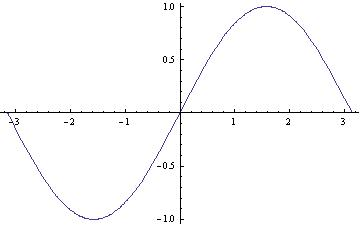
\includegraphics[height=2.5in, width=3.5in]{introduction/figures/sin_x.jpg}
\caption{Enjoyment and fun}
\end{figure}

Vestibulum ut urna eu turpis accumsan hendrerit. Mauris in mi sed eros auctor blandit. Nullam sit amet mauris vel eros aliquam pretium. Cras fermentum tortor. Sed egestas vulputate diam. Aenean sem dui, tincidunt a, ullamcorper eget, pharetra ac, tortor. In at sem vel elit bibendum convallis. Aenean ut enim vel leo malesuada dapibus. Etiam odio dolor, sollicitudin a, nonummy nec, tristique et, augue. Morbi ipsum. Aliquam venenatis. Proin orci. Duis sed quam eget turpis interdum feugiat.

\subsection{Hypothesis}  


Glossy prints of good reproducible quality, either black or white or color may be used. Photographs can be printed on 8 1/2$''$ x 11$''$ glossy finish paper, however, margin and page number requirements as stated above still apply for pages containing photographs. When attaching photographs to paper, double-sided tape may be used which causes the least amount of damage to the original paper.

The format of footnotes and the bibliography are to be prepared in accordance with standard practice in the field in which one is working. Documentation formatting style must be discussed with and accepted by the advisor. See further information on Reference Styles below.

The suggested typeface for dissertations is 10 to 12 point Arial. Other suggested fonts are Times New Roman and Helvetica. Script and italic fonts should not be used except as needed in the body of the paper. Consistency should be maintained throughout the paper, using the same font for all text, diagrams, etc. on all pages.

Electronic material, such as CDs and multimedia can accompany the dissertation. Each copy should be accompanied with a labeled CD. When bound, these are placed in an envelope in the back of the dissertation.  Oversized materials (pages greater than 8$''$ x 11$''$) can be included in the paper if necessary. Oversized pages should be folded so that 1$''$ on the left hand binding edge remains, allowing the page to be opened once the paper is bound.

The reference style used for formatting the paper must be confirmed with your department and advisor. Frequently used styles are the APA (American Psychological Association), MLA (Modern Language Association) and AMA (American Medical Association) styles. Style guides and manuals are available for each style. Page headers are not to be used.
